\documentclass[a4paper,12pt]{article}

\usepackage{amsmath,amssymb,amsthm,multicol,tikz,enumitem}
\usepackage{hyperref}
\usepackage[margin=2cm]{geometry}
\usepackage{fancyvrb}
\usetikzlibrary{calc}

\newcommand\N{\mathbf{N}}
\newcommand\Q{\mathbf{Q}}
\newcommand\R{\mathbf{R}}
\newcommand\Z{\mathbf{Z}}

\newcommand\rem{\textup{rem}}

% Comment out one or the other

\newcommand\answer[1]{}
\newcommand\ans[1]{}
\newcommand\anscommand[1]{}
%\newcommand\answer[1]{${}$\\[5pt]{\color{blue}{#1}}\hfill{\color{blue}$\qed$}\\[-5pt]} 
%\newcommand\ans[1]{{\color{blue}{#1}}}
%\newcommand\anscommand[1]{#1}


\begin{document}

\begin{center}
{\bf\Huge Exam 1} \\[5pt]
Data Structures \\
Thursday, October 7, 2021\\[5pt]
\textit{*You must justify all your answers to recieve full credit*}
\end{center}

\hrule
\vspace{2pt}
\hrule
\vspace{12pt}

% 1. C++ apart from Object Orientation
% 1.A. Restore/drop parentheses, use syntax trees.
% 1.B. Translate between flowcharts and C++ control structures. 
% 1.C. Use bit arithmetic.
% 1.D. Side-effects in operators, arrays, short-circuit Boolean evaluation.
% 1.E. Run pseudocode pointer operations, draw arrows.
% 1.F. (C++ code) Perform bit manipulation.
% 1.G. (C++ code) Manipulate arrays, char arrays (C-strings), 2D arrays.
% 1.H. (C++ code) Input data using "iostream", "sstream", "getLine", "get", "peek"

% 2. C++ with Object Orientation
% 2.A. Parameter passing to functions, "const" modifier, default parameters.
% 2.B. The order how constructors and destructors are executed.
% 2.C. (C++ code) Implement inheritance with virtual/non-virtual functions.
% 2.D. (C++ code) Custom comparison function to generic sorting, max or similar algorithm.

% 3. Big-O, Omega, Theta Notation
% 3.A. Find the asymptotic growth for a given function.
% 3.B. Compare classes of function growth or order them.
% 3.C. Express time complexity for recursively defined functions. 
% 3.D. Express time complexity for a code snippet ``from the inside out''. 
% 3.E. Find the amortized time complexity for an operation on a given data structure.
% 3.F. Count the number of calls for comparisons or similar functions.

% 4. Lists, stacks, queues.} 
% 4.A. Use Abstract Data Type (ADT) to write algorithms.
% 4.B. (C++ code) Use STL classes for lists, stacks, queues with iterators.


% "1C" "1E" "2B" "3A" "4B" 


\begin{enumerate}

%%%%%%%%
%% 01 %%
%%%%%%%%
\item 
% 1.C. Use bit arithmetic.

Consider a code fragment using the bitwise XOR.

\begin{Verbatim}[frame=single,numbers=left]
int a = -3;
int x = ???  // replace this ??? with a number
int b = a^x;
cout << hex << b;
// This outputs the hexadecimal representation of "b": "ffffabcd".
\end{Verbatim}


\begin{enumerate}
\item Write the hexadecimal representation of variable \texttt{a}, if its decimal value is $-3$.
\item Write the binary representation of the same variable \texttt{a}.
\item Write the hexadecimal representation of variable \texttt{x}. That is, rewrite line 2 of the code snippet above to make variable \texttt{b} equal to {\tt 0xffffabcd}. 
\end{enumerate}

\vfill

%%%%%%%%
%% 02 %%
%%%%%%%%
\item 
% 1.E. Run pseudocode pointer operations, draw arrows.

A doubly linked list has 3 structures of type {\tt Node} (see Figure~\ref{fig:nodes}): 
it has {\tt prev} and {\tt next} pointers of type {\tt Node*} 
and also a constant {\tt info} field storing constant positive integers. That is, the {\tt info} field does not change over the lifetime of the \texttt{Node}. 

\begin{figure}[!htb]
\center{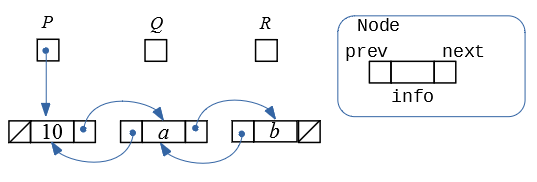
\includegraphics[width=4in]{ds-exam1/nodes.png}}
\caption{\label{fig:nodes} Doubly linked list}
\end{figure}

Variable {\tt P} is a pointer of type {\tt Node*}, 
initially {\tt P} points to the first node in this list. 
The {\tt info} fields in this list have values $10$, $a$ and $b$. 

Write code that modifies this doubly linked list in the following way:
\begin{itemize}
\item If $a > b$, the pointers in the list change so that the \texttt{Node} with \texttt{info} field value $10$ points to $b$ (that \texttt{Node} is now second), and the \texttt{Node} with \texttt{info} field $b$ points to $a$ (that \texttt{Node} is now third). 
\item If $a \leq b$, then your code should leave the list unchanged.
\end{itemize}

\vfill
\clearpage

%%%%%%%%
%% 04 %%
%%%%%%%%
\item \label{q:q4}
% 4.B. (C++ code) Use STL classes for lists, stacks, queues with iterators.

The following C++ program declares a class {\tt Pair}. 
Pairs are {\em lexicographically ordered}: 
\[
(x_1, y_1) < (x_2, y_2)\ \ \text{iff}\ \ x_1 < x_2\ \vee\ (x_1 = x_2\ \wedge\ y_1 < y_2).
\]
Complete the code below so that, when compiled and executed, in order:
\begin{itemize}
\item a positive integer $n$ is input,
\item $n$ pairs from the standard input are input,
\item the $n$ pairs are pushed on the stack, skipping pairs which are not lexicographically larger than the current top element of the stack,
\item the remaining pairs are output to the standard output as separate lines in their original order.
\end{itemize}

Use the overloaded operators ``{\tt cout << pair}'', ``{\tt cin >> pair}'', ``{\tt p1 < p2}''
for input, output and comparisons. The only data structure to use is STL stack. 
If necessary, you may use several stacks.

\begin{Verbatim}[frame=single,numbers=left]
#include <iostream>
#include <stack>
using namespace std;
class Pair { public: int x; int y; }; 
istream &operator>>(istream  &input, Pair &p ) { 
  input >> p.x >> p.y;   return input;            
}
ostream &operator<<(ostream &output, const Pair &p ) { 
  output << "(" << p.x << "," << p.y << ")";   return output;            
}
bool operator<(const Pair &left, const Pair &right) {
  // implement the lexicographic comparison operator.
}
int main() {
  // Input the total number of pairs, then 2*n integers (the pairs). 
  // Output those pairs which are in lexicographically increasing order.
}
\end{Verbatim}

{\bf Sample input}

\begin{Verbatim}[frame=single]
5
4 17
4 17
5 1000
7 12
7 9
\end{Verbatim}

{\bf Sample output}

\begin{Verbatim}[frame=single]
(4,17)
(5,1000)
(7,12)
\end{Verbatim}

\clearpage

%%%%%%%%
%% 05 %%
%%%%%%%%
\item 
% 2.B. The order how constructors and destructors are executed.
In your code from Question \ref{q:q4}, define the default (no argument) constructor, copy constructor 
and destructor. Describe the order in which these are called when your compiled code is executed with the input below.

\begin{Verbatim}[frame=single]
2
2 3
1 4
\end{Verbatim}

In your answer you should list the order how the constructors of both types (and also destructor)
are invoked for every {\tt Pair} object. Describe why this behavior makes sense 
and generalize -- how many invokations would happen for $n$ pairs in the input.


\vspace{1cm}

%%%%%%%%
%% 03 %%
%%%%%%%%
\item
% 3.A. Find the asymptotic growth for a given function.

Consider the functions $f_1(n)$, $f_2(n)$, $f_3(n)$, $f_4(n)$ below, mapping positive integers $n \geq 5$
to positive real numbers $t>0$: 
% n^3.5
% 
\begin{align*}
f_1(n) & = (1 + \cos n) \sqrt{2^{7 \cdot \log_2 (n)}},\\
f_2(n) & = 13^{\log_2 (n)},\\
f_3(n) & = \frac{1}{n^2} \cdot {n \choose 5},\\
f_4(n) & = f_1(n) + f_2(n) + f_3(n).
\end{align*}

For each function $f_i(n)$, $i=1,2,3,4$, find functions 
\begin{itemize}
\item $g_i(n)$ such that $f_i(n)$ is $O(g_i(n))$,
\item $h_i(n)$ such that $f_i(n)$ is $\Omega(h_i(n))$, 
\item $k_i(n)$ such that $f_i(n)$ is $\Theta(k_i(n))$. 
\end{itemize}
Give justifications for all your answers.


\end{enumerate}


\end{document}